\subsection{JiraGPT Next}
Partiendo del trabajo realizado por Joel García, se dispone de JiraGPT Next como una herramienta que ayuda a recuperar incidencias filtradas utilizando lenguaje natural. De esta manera, una persona que no posea conocimiento técnico en la generación de consultas JQL podrá filtrar incidencias facilmente. JQL es un lenguaje de consulta que permite recuperar incidencias de Jira de manera avanzada y precisa, pero que requiere conocimientos técnicos para su uso. 

Tras esta herramienta se encuentra una llamada de API a un LLM que, utilizando una plantilla para guiar al modelo, pedirá que se traduzca la pregunta en lenguaje natural a una consulta JQL que responda a lo que se pide.

Se puede apreciar una captura de la aplicación en la figura \ref{fig:estado_inicial}, que consiste en una ventana de chat en la que se puede interactuar con el asistente con varias opciones disponibles. La persona que lo utilizase, presumiblemente un gestor de proyectos que no conoce JQL y necesita información sobre el proyecto en Jira podría lanzar sus preguntas y obtener respuestas con un resumen y los campos que ha solicitado. Tendría varias opciones, como la temperatura, que representa lo 'creativo' que puede ser el modelo (más estocástico o determinista), la plantilla o el modelo a utilizar y un checkbox para activar la pregunta compleja, que seleccionaría los campos relevantes de la respuesta a la consulta JQL.

\begin{figure}[H]
    \centering
    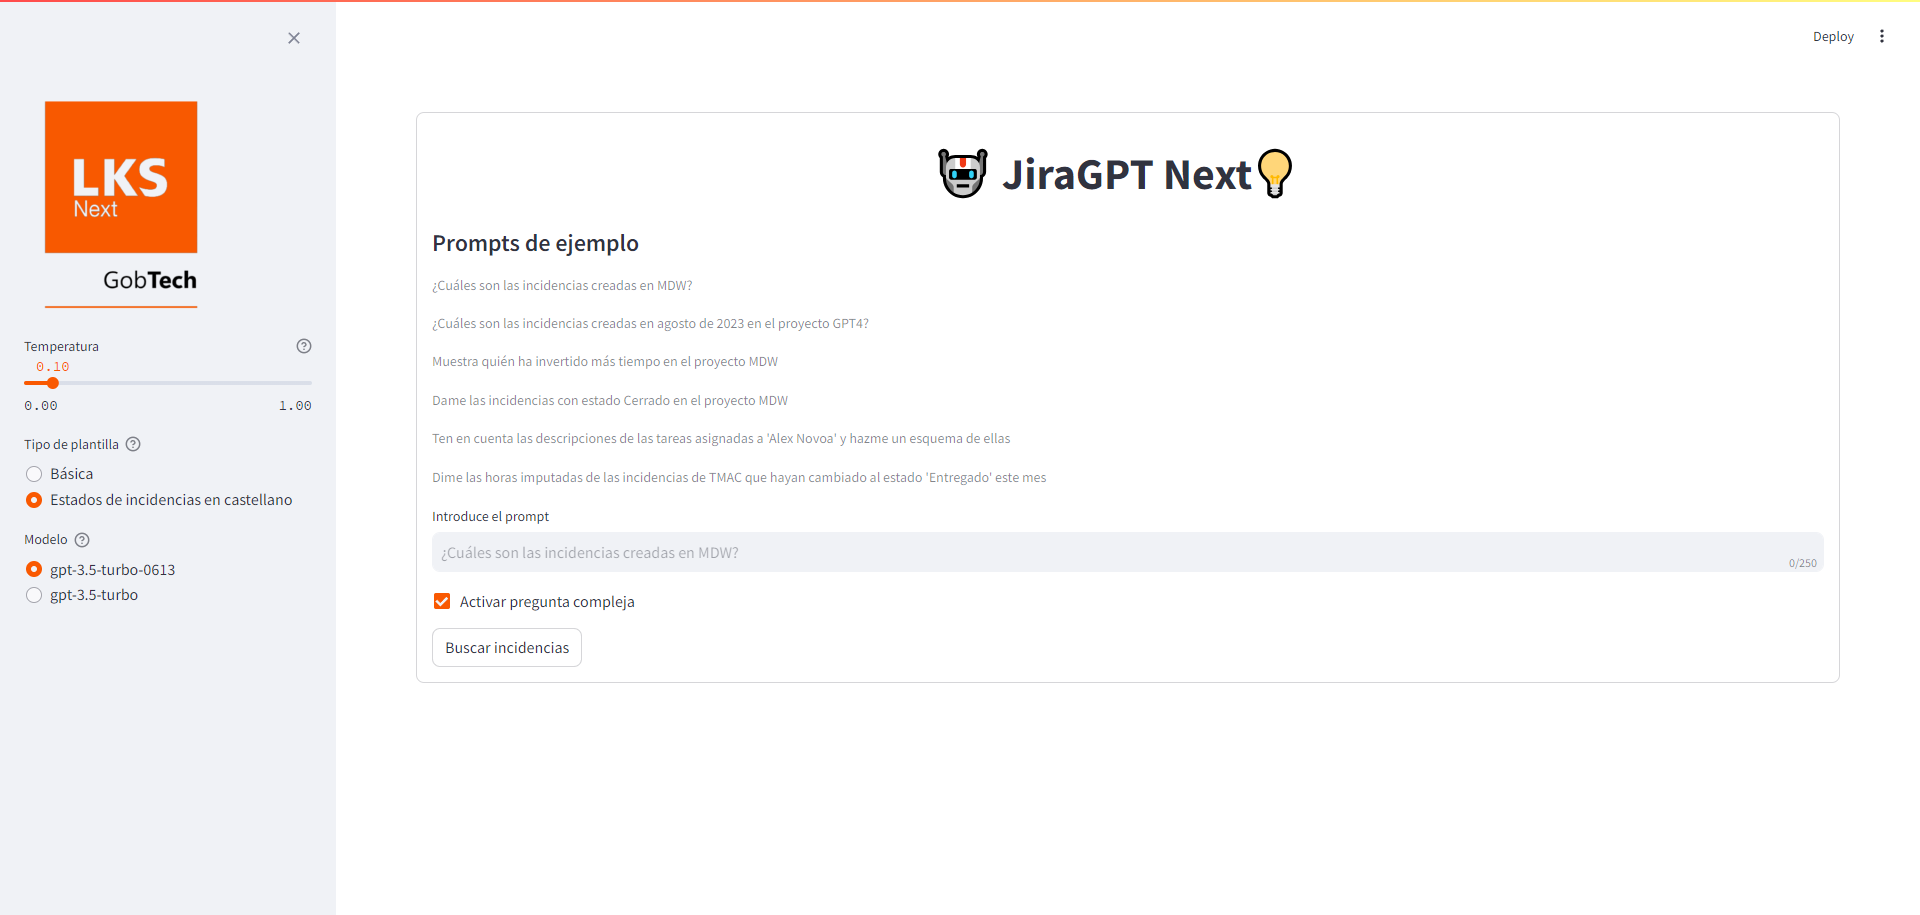
\includegraphics[width=0.95\textwidth]{images/Streamlit_inicial.png}
    \caption{Interfaz de la aplicación}\label{fig:estado_inicial}
\end{figure}

La idea de este nuevo trabajo es realizar un estudio del potencial cambio en precisión que se puede lograr utilizando técnicas de Retrieval Augmented Generation (RAG), entendiendo precisión como el número de preguntas que el sistema es capaz de responder correctamente. Para ello, se van a proponer tres implementaciones diferentes de una base de conocimiento de la que el modelo pueda aprovechar la información contenida para generar respuestas partiendo de un mayor contexto. 

